	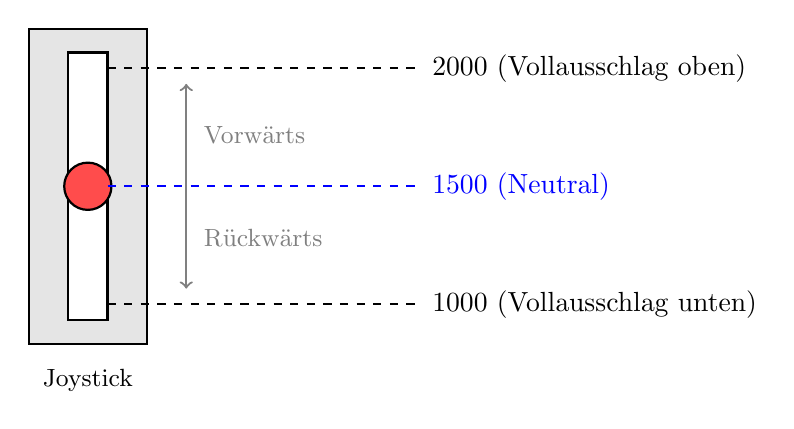
\begin{tikzpicture}
	% Joystick Gehäuse
	\draw[thick, fill=gray!20] (0,0) rectangle (1.5,4);
	
	% Joystick Slot (vertikale Führung)
	\draw[thick, fill=white] (0.5,0.3) rectangle (1.0,3.7);
	
	% Joystick Knopf in Mittelstellung
	\draw[thick, fill=red!70] (0.75,2.0) circle (0.3cm);
	
	% Beschriftung Joystick
	\node[below] at (0.75,-0.2) {\small Joystick};
	
	% Gestrichelte Linien mit Werten
	% Obere Position (2000 µs)
	\draw[dashed, thick] (1.0,3.5) -- (5,3.5);
	\node[right] at (5,3.5) {\SI{2000}{\micro\second} (Vollausschlag oben)};
	
	% Mittlere Position (1500 µs) - Neutralstellung
	\draw[dashed, thick, blue] (1.0,2.0) -- (5,2.0);
	\node[right, blue] at (5,2.0) {\SI{1500}{\micro\second} (Neutral)};
	
	% Untere Position (1000 µs)
	\draw[dashed, thick] (1.0,0.5) -- (5,0.5);
	\node[right] at (5,0.5) {\SI{1000}{\micro\second} (Vollausschlag unten)};
	
	% Pfeile für Bewegungsrichtung
	\draw[->, thick, gray] (2,2.0) -- (2,3.3);
	\node[right, gray] at (2.1,2.65) {\small Vorwärts};
	
	\draw[->, thick, gray] (2,2.0) -- (2,0.7);
	\node[right, gray] at (2.1,1.35) {\small Rückwärts};

	
\end{tikzpicture}